%version of 11-04-18

\chapter{NUMBERS II, BEYOND THE BASICS}
\label{ch:numbers-advanced}


\section{Prime Numbers: Building Blocks of the Integers}
\label{sec:primes}
\index{number!prime numbers}
\index{integers!prime numbers}

We single out a subclass of the positive integers whose mathematical
importance has been recognized for millennia but which have found
important new applications (e.g., within the domain of computer
security) as recently as within the past several decades.  This
subclass is defined by its divisibility characteristics.

Note that every positive integer $n$ is divisible by $1$ and by $n$.
The subclass of interest consist of those $n$ that have no other
divisors.

An integer $p >1$ is {\it prime}\index{number!integer!prime
  number}\index{number!integer!prime}\index{prime
  number}\index{integer!prime number}\index{integer!prime}
if its {\em only} positive integer divisors are $1$ (which divides
every integer) and itself (which is always a divisor).

\[ \approx \approx \approx \approx \approx \approx \approx \approx \approx \approx \]
{\em We often use the shorthand assertion, ``$p$ is a prime'' (or even
  the simpler ``$p$ is prime'') instead of the longer, but equivalent,
  ``$p$ is a prime integer.''}
\[ \approx \approx \approx \approx \approx \approx \approx \approx \approx \approx \]

  
\subsection{The Fundamental Theorem of Arithmetic}
\label{sec:Fund-Thm-Arith}

\subsubsection{Statement and proof}
\label{sec:FTA-basics}

A very consequential way to classify a positive integer $n$ is to list
the primes that divide it, coupling each such prime $p$ with its {\it
  multiplicity}, i.e., the number of times that $p$ divides $n$.  Let
$p_1, p_2, \ldots, p_r$ be all of the distinct primes that divide $n$,
and let each $p_i$ divide $n$ with multiplicity $m_i$.  The {\it prime
  factorization} \index{prime factorization} \index{integer!prime
  factorization} \index{number!integer!prime factorization}
of $n$ is the product $p_1^{m_1} \cdot p_2^{m_2} \cdot \cdots \cdot
p_r^{m_r}$; note that this product satisfies the equation
\begin{equation}
\label{eq:prime-factorization}
n \ = \ p_1^{m_1} \cdot p_2^{m_2} \cdot \cdots \cdot p_r^{m_r}
\end{equation}
When writing an integer $n$'s prime factorization, it is traditional
to write the factorization in {\it canonical form},
\index{prime factorization!canonical form}
\index{integer!prime factorization!canonical form}
\index{number!integer!prime factorization!canonical form}
i.e., with the primes $p_1, p_2, \ldots, p_r$ that divide $n$ listed
in increasing order, i.e., so that $p_1 < p_2 < \cdots < p_r$.

A positive integer $n$ is totally characterized by its canonical prime
factorization, as attested to by the following classical theorem,
which has been known for millennia and has been honored with the title
{\em The Fundamental Theorem of Arithmetic}.
\index{Fundamental Theorem of Arithmetic}
We state the Theorem in two equivalent ways which suggest somewhat
different ways of thinking about the result.

\begin{theorem}[The Fundamental Theorem of Arithmetic]
\index{Fundamental Theorem of Arithmetic}
\label{thm:Fund-Thm-Arith}

\noindent
{\rm (Traditional formulation.)}
%
The canonical prime factorization of every positive integer is unique.

\noindent
{\rm (Alternative formulation.)}
%
Let $n \in \N^+$ be a positive integer, and let $\widehat{P}_n$ denote the
ordered sequence of prime numbers that are no larger than $n$:

\begin{tabular}{ll}
$\widehat{P}_n \ =$  & $\langle P_1, \ P_3, \ \ldots, \ P_{r-1}, \ P_r \rangle$ \\
where:               & $P_1 \ = \ 2$ \\
                     & each  \ \ $P_i \ < \ P_{i+1}$ \\
                     & $P_r \ \leq \ n$.
\end{tabular}

\noindent
There exists a unique sequence of {\em nonnegative} integers, 
$\langle a_1, a_2, \ldots, a_r \rangle$
such that
\[
n \ = \ \prod_{i=1}^r \ P_i^{a_i} \ = \
P_1^{a_1} \cdot P_2^{a_2} \cdot \ \cdots \ \cdot P_{r-1}^{a_{r-1}} \cdot P_r^{a_r}
\]
\end{theorem}

A simple, yet important, corollary of Theorem~\ref{thm:Fund-Thm-Arith}
is the following result, whose proof we leave to the reader.

\begin{prop}
\label{thm:prime-divisor}
Every integer $n>1$ is divisible by at least one prime number.
\end{prop}

\bigskip

\noindent {\it Proving the Fundamental Theorem of Arithmetic.}
%
The proof of Theorem~\ref{thm:Fund-Thm-Arith} is actually rather
elementary, providing that one approaches it gradually.  It employs a
lot of important techniques and concepts involved in ``doing
mathematics'', as discussed in the eponymous
Chapter~\ref{ch:doingmath}.

We begin with a purely technical result.

\begin{prop}
\label{thm:p-n-linear}
Let $p$ be a prime, and let $m$ be any positive integer that is {\em
  not} divisible by $p$.  There exist integers $a, b$, not necessarily
positive, such that
\[ ap + bm \ = \ 1. \]
\end{prop}

\begin{proof}
This result is a special case of Proposition~\ref{thm:gcd-n-linear}
because for any prime $p$ and integer $m$ that is not divisible by
$p$, {\sc gcd}$(p, m) = 1$.
\qed
\end{proof}

\begin{prop}
\label{thm:p-divides-onefactor}
If the prime $p$ divides a composite number $m \cdot n$, then either
$p$ divides $m$, or $p$ divides $n$, or both.\footnote{The closing
  phease ``or both'' signals our use of the {\em inclusive} or.}
\end{prop}

\begin{proof}
Let $p$, $m$, and $n$ be as asserted, and say that $p$ does not divide
$m$.  By Proposition~\ref{thm:p-n-linear}, then, there exist integers
$a, b$, not necessarily positive, such that
\[ ap + bm \ = \ 1. \]
Let us multiply both sides of this equation by $n$.  After some
manipulation---specfically, applying the distributive law---we find
that
\[ apn + bmn \ = \ n. \]
Now, $p$ divides the expression to the left of the equal sign: $p$
divides $p$ by definition, and $p$ divides $mn$ by assumption.  It
follows that $p$ must divide the expression to the right of the equal
sign---namely, the integer $n$.  \qed
\end{proof}

We are finally ready to develop the proof of the Fundamental Theorem.

\begin{proof}
{\small\sf The Fundamental Theorem of Arithmetic.}
%
Our dominant tool for proving Theorem~\ref{thm:Fund-Thm-Arith} will be
{\em proof by contradiction} (see Chapter~\ref{sec:Contradiction}).
We assume, for the sake of contradiction, that there is a positive
integer $n$ that has two distinct canonical prime factorizations.

Our argument will be a trifle simpler if we employ the {\em alternative} 
form of the Theorem.  To this end, let
\[ P_1 \ < \ P_2 \ < \cdots < \ P_{r-1} \ < \ P_r \]
denote, in increasing order, the set of all primes that do not exceed
$n$; i.e., every $P_i \leq n$.

The fact that $n$ has two distinct canonical prime factorizations
manifests itself, in this formulation, by the assumption that there
exist {\em two} distinct sequences of {\em nonnegative} integers, 
\[ \langle a_1, a_2, \ldots, a_r \rangle \ \ \ \mbox{ and } \ \ \
\langle b_1, b_2, \ldots, b_r \rangle 
\]
such that $n$ is expressible by---i.e., is equal to---both of the
following products of the primes $P_1$, $P_2$, \ldots, $P_{r-1}$, $P_r$.
\begin{eqnarray}
 & & 
\label{eq:product1.1}
P_1^{a_1} \cdot P_2^{a_2} \cdot \ \cdots \ \cdot P_{r-1}^{a_{r-1}}
\cdot P_r^{a_r} \\
 & &
\label{eq:product2.1}
P_1^{b_1} \cdot P_2^{b_2} \cdot \ \cdots \ \cdot P_{r-1}^{b_{r-1}}
\cdot P_r^{b_r}
\end{eqnarray}

Let us now ``cancel'' from the products (\ref{eq:product1.1}) and
(\ref{eq:product2.1}) the longest common prefix.  Because the two
products are, by hypothesis, distinct, at least one of them will not
be reduced to $1$ by this cancellation.  We are, therefore, left with
residual products of the forms
\begin{eqnarray}
 & &
\label{eq:product1.2}
P_i^{a_i} \cdot X \\
 & &
\label{eq:product2.2}
P_i^{b_i} \cdot Y
\end{eqnarray}
where:
\begin{itemize}
\item
Precisely one of $a_i$ and $b_i$ equals $0$.

Say, with no loss of generality (because we have no intrinsic way to
distinguish the products), that $b_i =0$ while $a_i \neq 0$.

\item
Products $X$ and $Y$ are composed only of primes that are strictly
bigger than $P_i$.
\end{itemize}
Note that 
\[ P_i^{a_i} \cdot X \ = \ P_i^{b_i} \cdot Y \ = \ Y, \]
because these products result from cancelling the same prefix from the
equal products (\ref{eq:product1.1}) and (\ref{eq:product2.1}), and
because $b_i =0$ so that $P_i^{b_i} = 1$.

We have finally reached the point of contradiction.

On the one hand, $P_i$ {\em must} divide the product $Y$, because it
divides the product $P_i^{a_i} \cdot X$ which equals $Y$.

On the other hand, $P_i$ {\em cannot} divide the product $Y$, because
every prime factor of $Y$ is bigger than $P_i$ (and a prime cannot
divide a bigger prime).

We conclude that one of the products (\ref{eq:product1.1}) and
(\ref{eq:product2.1}) cannot exist, so the theorem must hold.  \qed
\end{proof}


\subsubsection{A ``prime'' corollary: There are infinitely many primes}
\label{sec:infinite-primes}

The main result of this section, which is traditionally attributed to
(our friend, by now) Euclid, \index{Euclid}, invokes
Theorem~\ref{thm:Fund-Thm-Arith} in a crucial way.

\begin{prop}
\label{thm:infinite-primes}
There are infinitely many prime numbers.
\end{prop}

\begin{proof}
We know that the first several primes are
\[ (P_1 =2), \ (P_2 = 3), \ (P_3 =5), \ (P_4 = 7), \ (P_5 =11), \ldots \] 
How far does this sequence extend?  Does it ever end?

Let us assume, for the sake of contradiction, that there are only
finitely many primes (so that our sequence ends).  Say, in particular,
that the following $r$-element sequence of integers enumerates all
(and only) primes, in order of magnitude:

$ \begin{array}{ccl}
\mbox{\bf Prime-Numbers} & = & 
\langle P_1, \ P_2, \ \ldots, \ P_r \rangle \\
\mbox{ where} &  &
P_1 \ < \ P_2 \ < \cdots < \ P_{r-1} \ < \ P_r
\end{array}
$

\medskip

We verify the {\em falseness} of the alleged completeness of the sequence
{\bf Prime-Numbers} by analyzing the positive integer
\[ n^\star \ = \ 1 + \prod_{i=1}^r \ P_i \ = \ 1 \ + \ 
\left(P_1 \cdot P_2 \cdot \cdots \cdot P_r \right).
\]

In fact, we claim that $n^\star$ is a prime that is not in the
sequence {\bf Prime-Numbers}.  We begin to verify our claim by making
three crucial observations.
\begin{enumerate}
\item
{\em The number $n^\star$ is not divisible by any prime in the sequence}
{\bf Prime-Numbers}.

To see this, note that for each $P_k$ in the sequence,
\[
n^\star / P_k \ \ = \ \ \frac{1}{P_k} \ + \ \prod_{i \neq k} \ P_i .
\]
Because $P_k \geq 2$, we see that $n^\star / P_k$ obeys the inequalities
\[
\prod_{i \neq k} \ P_i \ < \ n^\star /P_k \ < \ 1 + \prod_{i \neq k} \ P_i.
\] 
The discreteness of the set $\Z$---see
Section~\ref{sec:integer-number-line}---implies that $n^\star / P_k$ is not
an integer, because it lies strictly between two adjacent integers.

\item
Because of observation 1, if the sequence {\bf Prime-Numbers} actually
did contain {\em all} of the prime numbers, then we would have to
conclude that {\em the number $n^\star$ is not divisible by any prime
  number.}

\item
Finally, we remark that the Fundamental Theorem of Arithmetic
(Theorem~\ref{thm:Fund-Thm-Arith}) implies that {\em every integer $m
  >1$ is divisible by (at least one) prime number}.
\end{enumerate}
The preceding chain of assertions leads to a mutual inconsistency.  On
the one hand, the integer $n^\star >1$ has no prime-integer divisor.
On the other hand, no such integer can fail to have a prime-integer
divisor!

Let us analyze how we arrived at this uncomfortable place.
\begin{itemize}
\item
At the front end of this string of assertions we have the assumption
that there are only finitely many prime numbers.  We have (as yet) no
substantiation for this assertion.
\item
At the back end of this string of assertions, we have the ({\em rock
  solid}) Fundamental Theorem of Arithmetic
(Theorem~\ref{thm:Fund-Thm-Arith}).
\item
In between these two assertions we have a sequence of assertions, each
of which follows from its predecessors via irrefutable rules of
inference.
\end{itemize}
It follows that the {\em only} brick in this edifice that could be
faulty---i.e., the only assertion that could be false---is the initial
assumption, which states that there are only finitely many prime
numbers.  {\em We must, therefore, conclude that this vulnerable
  assumption is false!}  In other words, we conclude from this
classical proof by contradiction that there are infinitely many prime
numbers.  \qed
\end{proof}


\subsubsection{Applying the Theorem in {\em encryption}}
\label{sec:apply-FTA}

One of the most important applications of Theorem~\ref{thm:Fund-Thm-Arith} is
as a mechanism for facilitating {\em encryption}.
\index{number!using the Fundamental Theorem of Arithmetic for encoding}
\index{number!using prime numbers for encoding}
\index{encoding sequences via the Fundamental Theorem of Arithmetic}
%
While the details of both encryption and the use of prime numbers to
that end are beyond the scope of this text, we will provide a peek
into that area by means of the following result concerning {\it
  encodings} of sequences of positive integers as single integers!

\[ \approx \approx \approx \approx \approx \approx \approx \approx \approx \approx \]
There is a crucial difference between {\em encoding} and {\em
  encryption}, despite the words' often being confused in the
vernacular.

Encodings seek representations of objects which achieve some benefit,
such as efficient computation or compactness.  An example might be the
conversion of Roman numerals to positional numerals to enhance the
arithmetic operations.

Encryption usually has some notion of secrecy attached.  An example
might be some key-based cipher which is intended to limit access to
some information.
\[ \approx \approx \approx \approx \approx \approx \approx \approx \approx \approx \]

We illustrate (and achieve) the sought encodings as follows.  Consider
the (infinite) ordered sequence of {\em all primes:}
\[ (P_1 = 2), (P_2 = 3), (P_3 = 5), \ldots  \]
Let
\begin{equation}
\label{eq:sequence-vec-s}
\bar{s} \ \ = \ \ \langle m_1, m_2, \ldots, m_k \rangle
\end{equation}
be an arbitrary sequence of positive integers.  Then
Theorem~\ref{thm:Fund-Thm-Arith} assures us that the (single) positive
integer
\[ 
\iota(\bar{s}) \ \ = \ \ P_1^{m_1} \cdot P_2^{m_2} \cdot \ \cdots \
\cdot P_k^{m_k}
\]
is a (uniquely decodable) integer-representation of sequence $\bar{s}$.

We return to this idea of encoding-via-integers in a later chapter.

\subsubsection{Enrichment: The ``density'' of the prime numbers}
\label{sec:prime-density}

{\Arny There are two advanced topics that we may want to
  mention/discuss: (1) The prime-number theorem ($n/ \log n$ primes
  $\leq n$); (2) the polynomials that generate lots of primes.  We
  should discuss this}
  

\subsection{Fermat's Little Theorem}
\label{sec:fermat}
\index{Fermat's Little Theorem}

A measure of the greatness of the 17th-century French mathematician
Pierre de Fermat \index{Fermat, Pierre de} is that the following
fundamental result is called his ``little theorem.''  Aside from its
exposing an important and basic property of prime numbers, the theorem
provides the basis for a valuable algorithm for testing the primality
of integers.


\begin{theorem}[Fermat's Little Theorem]
\index{Fermat's Little Theorem}
\label{thm:Fermat's-Little-Thm}

Let $a$ be any integer, and let $p$ be any prime.

{\rm (Formulation 1):}
The number $a^p \ − \ a$ is divisible by $p$.

\medskip

{\rm (Formulation 2):}
$a^{p} \equiv a \bmod p$.
\end{theorem}

%Notice that there exist other formulations, the following is the most popular one:
%
%Let consider two primes $p$ and $a$.
%$a^{p-1} \equiv 1 [p]$

\noindent
We provide two proofs for this fundamental result, each providing
rather different insights on the result.


\subsubsection{A proof using ``necklaces''}
\label{sec:FTL-necklaces}

\begin{proof}
The idea underlying this proof is to design a framework in which the
result can be reduced to counting a special set of strings.

Letting $a$ and $p$ be as in the theorem, consider the set $S(\a,p)$ of
all words/strings of length $p$ over an alphabet/set $\a = \{ \alpha_1,
\alpha_2, \ldots, \alpha_a \}$ of $a$ symbols.  For instance, when $\a
= \{0,1\}$ (so that $a=2$) and $p=3$, the set $S(\a,p)$ consists of the
words:
\[ 000, \ 001, \ 010, \ 011, \ 100, \ 101, \ 110, \ 111 \]
We begin with some basic definitions and observations.
\begin{itemize}
\item
The number of words in $S(\a,p)$ is $a^p$; see
Proposition~\ref{thm:Num-strings-lgth-k}.

\item
A {\it (one-place) circular shift} $c$ of a word in $S(\a,p)$ is
accomplished by placing the last symbol of this word into the first
position and shifting all other symbols one position rightward.  For
illustration:
\[ c(\alpha_1 \alpha_2 \cdots \alpha_p) \ = \ \alpha_p \alpha_1 \cdots
\alpha_{p-1} \]
%Graph of $c$ for words of length $p=3$ on $\mathcal{A} = \{0,1\}$.

\item
By iterating the shift $c$ on a length-$p$ word $w$ at most $p-1$
times, we obtain the {\it necklace} $\n(w)$, which is the sequence
\[ \n(w) \ = \ w, \ c(w), \ c(c(w), \ldots, \ c(\cdots c(w)) \cdots )) \]
in which one further shift would replicate word $w$.

\item
The {\it period} of the necklase $\n(w)$ is the number of words in the
sequence.

Note that {\em the period of $\n(w)$ can never exceed $p-1$}---because
an earlier-seen word must recur by the time the length-$p$ word $w$
has been shifted $p$ times.
\end{itemize}

Consider now a word $w$ that is a {\it replicate}
\index{word!replicate} of another word $u$, in the sense that $w = uu
\cdots u$.  Say that $u$ is the shortest word of which $w$ is a
replicate and that $u$ has length $m$.  Then:
\begin{itemize}
\item
{\em $u$'s length $m$ divides $p$.}

This is obvious from our ability to write $w$ in the indicated form.

\item
{\em The period of $\n(w)$ is $m-1$.}

This is because, by the time one has shifted $w$ $m$ times, one has
transferred a copy of $u$ from the end of $w$ to the beginning.
Hence, one has recreated $w$.

\item
In our special situation---where $w$ has prime length---{\em The only
  candidates for the shortest replicated word $u$ have length $1$ or
  $p$.}

This is because $m$ divides the prime $p$.
\end{itemize}
Summing up, one of the following two situations must hold.

\noindent
Possibility \#1:
{\em The word $w$ has the form $w = \alpha \alpha \cdots \alpha$ for
  some symbol $\alpha \in \a$.}

This can occur in $a$ distinct ways because of $\a$'s cardinality..

\noindent
Possibility \#2:
{\em The word $w$ is not a replicate of any shorter word.}

Because $p$ is a prime, this possibility must hold for every one of
the $a^p - a$ words over $\a$ that contains at least $2$ distinct
symbols.  Because the period of any necklace $\n(w)$ for a word that
contains at least $2$ distinct symbols is exactly $p-1$, the lengths
of such necklaces must be exactly $p$.

This means that the $a^p - a$ words that each contain at least $2$
distinct symbols partition $S(\a, p)$ into disjoint sets of size $p$
each.  This, in turn, means that $p$ divides $a^p - a$.
\qed
\end{proof}

The reader's comprehension of this multi-step proof might be enhanced
by Figs.~\ref{fig:necklace3} and~\ref{fig:necklace24}.
\begin{figure}[ht]
\begin{center}
        \includegraphics[scale=0.3]{FiguresArithmetic/Necklace3.png}
        \caption{The 3 necklaces composed of the the same symbol ($a=3$)}
        \label{fig:necklace3}
\end{center}
\end{figure}
\begin{figure}[ht]
\begin{center}
        \includegraphics[scale=0.25]{FiguresArithmetic/Necklace24.png}
        \caption{Eight groups of necklaces of size $p=3$ (for $a=3$).}
        \label{fig:necklace24}
\end{center}
\end{figure}
These figures jointly depict all necklaces $\n(w)$ for $(p=3)$-letter
words over the alphabet $\a = \{ A,B,C \}$.  Fig.~\ref{fig:necklace3}
depicts the necklaces for words that use only a single letter;
Fig.~\ref{fig:necklace24} depicts the necklaces for words that use at
least two distinct letters.


\subsubsection{A proof using the Binomial Theorem}
\label{sec:FTL-via-BinomialTheorem}

\begin{proof}
Our next proof employs Formulation 2 of the Proposition.  We focus on
a fixed prime $p$ and argue by induction on the alphabet size $a$,
that $a^{p} \equiv a \bmod p$.

\noindent
{\it Base of the induction.}
The base case $a=1$ is straightforward because $1^{p} = 1$

\noindent
{\it Inductive hypothesis.}
We assume for induction that $a^{p} \equiv a \bmod p$ for all alphabet
sizes not exceeding the integer $b$.

\noindent
{\it Extending the induction.}
Invoking the restricted form of the Binomial Theorem,
we know---see (\ref{eq:restricted-binomial-thm})---that
\begin{equation}
\label{eq:FLT-0}
(b+1)^p \ = \ \left( b^p + 1 \right) \ + \
 \sum_{i=1}^{p-1} {p \choose i} b^{p-i}
%\ \ = \ \  \sum_{j=1}^{p-1} {p \choose {p-j}} b^j
\end{equation}
Pondering this equation, we make two important observations.

\noindent {\bf 1.}
We learn from the development in
Section~\ref{sec:binomial-coeff+Pascal}.C that $p$ divides all
``internal'' binomial coefficients, i.e., all coefficients
$\displaystyle {p \choose i}$ with $0 < i < p$.  This means that there
exists an integer $n_1$ such that
\begin{equation}
\label{eq:FLT-1}
 \sum_{i=1}^{p-1} {p \choose i} b^{p-i} \ = \ p \cdot n_1.
\end{equation}

\[ \approx \approx \approx \approx \approx \approx \approx \approx \approx \approx \]
As an aside, one can observe the just-exposed divisibility property of
``internal'' binomial coefficients by looking at Pascal's triangle;
see the rows corresponding to primes---i.e., rows $n=2$, $n=3$, and
$n=5$---in the triangle of Fig.~\ref{fig:TrianglePrime}.  (Remember
that rows are indexed beginning with $n=0$.)
\begin{figure}[ht]
\begin{center}
  \includegraphics[scale=0.3]{FiguresArithmetic/TrianglePascalPrimes.png}
\caption{The rows of Pascal's triangle that correspond to $n=0$,
  $n=1$, \ldots, $n=6$.  The ``internal'' entries of the rows that
  correspond to prime numbers---in this case, $n=2$, $n=3$, and $n=5$---are
  divisible by that number.}
\label{fig:TrianglePrime}
\end{center}
\end{figure}
\[ \approx \approx \approx \approx \approx \approx \approx \approx \approx \approx \]

\noindent {\bf 2.}
By the inductive hypothesis, $p$ divides $b^p -b$, which means that
there exists an integer $n_2$ such that
\begin{equation}
\label{eq:FLT-2}
 b^p \ = \ b \ + \ p \cdot n_2.
\end{equation}

\smallskip

When we combine relations (\ref{eq:FLT-1}) and (\ref{eq:FLT-2}), and
we use them to rewrite equation (\ref{eq:FLT-0}), we find that
\[
(b+1)^p \ = \ (b + 1) \ + \ p \cdot (n_1 + n_2).
\]
This means that $p$ divides $(b+1)^p \ - \ (b + 1)$, which extends the
induction and completes the proof.
\qed
\end{proof}

\ignore{********************
\paragraph{\small\sf C. A proof using Pascal's triangle}

Before presenting the proof, let us first establish a preliminary property:
\medskip

\noindent \textbf{Property.} 
\label{prop:preliminaryFermat}



Looking from another perspective (with Pascal triangles modulo primes) evidences this property. 
We detail it on two particular examples in Figures~\ref{fig:TriangleModulo5} and \ref{fig:TriangleModulo7} (namely, for $p=5$ and $p=7$). 

%Let us compute the powers of $p=7$ for the first successive integers:
%
%$1^7  \equiv 1 [7]$
%
%$2^7 = 128 = 7 \times 18 + 2  \equiv 2 [7]$
%
%$3^7 = 2187 = 7 \times 312 + 3 \equiv 3 [7]$
%
%$4^7 = 16 384 = 7 \times 2340 + 4 \equiv 4 [7]$
%
%$5^7 = 78 125 = 7 \times 11140 + 5  \equiv 5 [7]$
%
%$6^7 = 279 936  = 7 \times 39 990 + 6 \equiv 6 [7]$
%\bigskip

This result reflects the core of the little Fermat Theorem, that is:
\textbf{the reminders by a prime of a number and its power to the same
  prime remain the same}.  It can be proved formally by simply
applying the definition:

${p}\choose{k}$ $= \frac{p!}{k!(p-k)!}$ (for $0 < k < p$)

Thus,  $k!$ ${p}\choose{k}$ $= p(p-1)\cdots(p-k+1)$.

In other words, $p$ divides the product $k!$ ${p}\choose{k} $ but it
has no common divisor with $k!$ since $k < p$, thus, $p$ divides
${p}\choose{k}$.
\medskip

\begin{figure}[ht]
\begin{center}
        \includegraphics[scale=0.2]{FiguresArithmetic/TrianglePascalModulo5init.png}
         \includegraphics[scale=0.2]{FiguresArithmetic/TrianglePascalModulo5.png}
        \caption{Pascal triangle modulo a prime (here $p=5$) and its reproducible pattern.}
        \label{fig:TriangleModulo5}
\end{center}
\end{figure}

\begin{figure}[ht]
\begin{center}
        \includegraphics[scale=0.3]{FiguresArithmetic/TrianglePascalModulo7.png}
        \caption{Pascal triangle modulo a prime ($p=7$)}
        \label{fig:TriangleModulo7}
\end{center}
\end{figure}
******************}


\subsection{Mersenne Primes and Perfect Numbers}
\label{sec:perfect-numbers+Mersenne-primes}
\index{perfect numbers}
\index{number!integer!perfect}

This short section is dedicated to two related topics whose intrinsic
charm has garnered attention from mathematicians who study numbers and
their properties for more than three millennia.  The section is placed
here because of the central role of a particular class of prime
numbers in the story we relate here.

\subsubsection{Perfect numbers}
\label{sec:perfect-numbers}

Hearkening back to the ancient Greeks' mystical affinity for special
classes of integers, we term a positive integer $n \in \N^+$ {\it
  perfect} 
\index{number!perfect}\index{number!integer!perfect}\index{perfect number} 
if $n$ equals the sum of its proper divisors.\footnote{Euclid refers
  to perfect numbers in his {\it Elements}, using adjectives such as
  ``perfect'' and ``ideal.''}  \index{Euclid}
It is not intuitive that perfect numbers even exist, but only a short
search is needed until one realizes that
\[ 6 \ \ = \ \ 1 \cdot 2 \cdot 3 \ \ = \ \ 1 \ +\ 2 \ + \ 3 \]
A few more minutes will lead one to the double equation
\[ 28  \ \ = \ \ 1 \cdot 2 \cdot 4 \cdot 7 \cdot 14
  \ \ = \ \ 1 \ + \ 2 \ + \ 4 \ + \ 7\ + \ 14 \]
It may take a bit longer, but the curious reader will eventually
discover the double equation
\begin{eqnarray*}
496 & = & 
1 \cdot 2 \cdot 4 \cdot 8 \cdot 16 \cdot 31 \cdot 62 \cdot 124 \cdot
248 \\
 & = &
1 \ + \ 2 \ + \ 4 \ + \ 8 \ + \ 16 \ + \ 31 \ + \ 62 \ + \ 124 \ + \ 248
\end{eqnarray*}

You may have absorbed enough of our ``How to be a mathematician'' lore
by this point to ask the following ``natural'' (to a mathematician, at
least) questions.

\smallskip

\begin{tabular}{l}
{\bf Question \#$1$.}  {\em Are there {\em infinitely many} perfect numbers?} \\
{\bf Answer.}  We imminently derive a positive response. \\
 \\
{\bf Question \#$2$.}  {\em Are there any {\em odd} infinitely many perfect numbers?} \\
{\bf Answer.}  No one knows---as of 2018.
\end{tabular}

\subsubsection{Mersenne primes}
\index{Mersenne prime}
\index{integer!prime!Mersenne prime}
\label{sec:Mersenne-primes}

A prime number $p$ is a {\it Mersenne prime}---so named for the
17th-century French monk Marin \index{Mersenne prime}
\index{integer!prime!Mersenne prime} Mersenne---if it has the form $p
= 2^q -1$ for some integer $q$.  It is obvious that Mersenne primes
exist: to wit,
\begin{equation}
\label{eq:sample-mersennes}
\begin{array}{lclc}
\mbox{The number} & p=3 & 
  \mbox{is a Mersenne prime, because} & 3 \ = \ 2^2 -1 \\
\mbox{The number} & p=7 &
  \mbox{is a Mersenne prime, because} & 7 \ = \ 2^3 -1 \\
\mbox{The number} & p=31 &
  \mbox{is a Mersenne prime, because} & 31 \ = \ 2^5 -1
\end{array}
\end{equation}
(There are obviously primes---such as $5$ and $13$---that are not
Mersenne primes.)  Despite the promising beginning to our list, we
cannot extend it too far: To wit, only about $50$ Mersenne primes are
known!  Indeed, it is not known---as of 2018---whether there exist
infinitely many Mersenne primes!  It is true, though, that {\em
  largest known prime}---as of 2018---{\em is a Mersenne prime:}
$2^{77,232,917} -1$.  \index{integer!prime!largest known} We close our
discussion of Mersenne primes as an isolated topic---i.e., unrelated
to perfect numbers---with the following result, which limits one's
search for Mersenne primes to expressions with prime powers of $2$.

%corollary of Fermat's Little Theorem (Theorem~\ref{thm:Fermat's-Little-Thm}).

\begin{prop}
\label{thm:Mersenne-needs-prime-exponent}
The integer $2^q -1$ is prime only if the integer $q$ is prime.
\end{prop}

\begin{proof}
Say, for contradiction, that there is a composite number $q = m \cdot
n$, with both $m, n > 1$, such that $2^q -1$ is a prime.  We invoke
identity (\ref{eq:geom-sum:b>1}) from
Proposition~\ref{thm:sum-finite-geometric-series} to show that $2^q
-1$ is, in fact, {\em not} prime.  We note, by direct calculation,
that
\begin{eqnarray}
\nonumber
2^{m \cdot n} -1 & = & (2^m -1) \cdot \frac{2^{m \cdot n} -1}{2^m -1} \\
\nonumber
  & = & (2^m -1) \cdot \sum_{i=0}^{n-1} \ \ (2^m)^{i} \\
\label{eq:Mersenne-factors}
  & = & (2^m -1) \cdot \left( 1 \ + \ (2^m) \ + \ (2^m)^2 \ + \cdots
            \ + \ (2^m)^{n-1} \right)
\end{eqnarray}
The number $r = 2^q - 1$ is, thus the product of two numbers, both
greater than $1$ and less than $r$, hence is not a prime.
\qed
\end{proof}

\subsubsection{Using Mersenne prime to generate perfect numbers}
\label{sec:MP+PN}

We unite the subjects of the preceding two subsections to derive the
basis of a procedure that employs Mersenne primes to generate perfect
numbers.

Let us revisit the three sample perfect numbers presented at the
beginning of Section~\ref{sec:perfect-numbers}.  As the following
table illustrates, all three numbers share the form $2^{p-1} \cdot
(2^p -1)$, where both $p$ and $2^p-1$ are primes.
\[ \begin{array}{ccrcrcccccc}
n & = & 6   & = & 2 \cdot 3  & = & 2^1 \cdot (2^2 -1) & 
\mbox{ so that } & p = 2 & 
\mbox{ and } & 2^p-1 = 3 \\
n & = & 28  & = & 4 \cdot 7  & = & 2^2 \cdot (2^3 -1) & 
\mbox{ so that } & p = 3 &
\mbox{ and } & 2^p-1 = 7 \\
n & = & 496 & = & 16 \cdot 31 & = & 2^4 \cdot (2^5 -1) & 
\mbox{ so that } & p=5 &
\mbox{ and } & 2^p-1 = 31
\end{array}
\]
It was no accident that the three perfect numbers we found have
intimate formal relationships with the first three primes.  In fact,
the result we present now establishes that every Mersenne prime has
such a formal relationship with a perfect number---thereby providing
us the promised path toward generating perfect numbers.\footnote{This
  result (of course with no mention of Mersenne) appears in Euclid's
  \textit{Principae IX-36}. \index{Euclid}}

\begin{prop}
\label{thm:MP-PN}
For every Mersenne prime $2^p-1$, the number
\begin{equation}
\label{eq:Mersenne-perfect-p}
2^{p-1} \cdot (2^p-1) \ = \ {{2^p} \choose 2}
\end{equation} 
is perfect.
\end{prop}

\begin{proof}

The list of factors $F_i$ (for $0 \leq i \leq \alpha-1$) of $2^{\alpha-1}$ is: 

$F_0=1, F_1=2, F_2=4, ..., F_{\alpha-1}=2^{\alpha-1}$.

The other factors of $PN_\alpha$ are obtained by: $F_i.(2^\alpha-1)$ for $i < \alpha-1$.

Summing up all these factors, we obtain:

$\Sigma_{i=0,\alpha-1} 2^{i} + \Sigma_{i=0,\alpha-2} 2^{i}(2^\alpha-1)$

$= 2^{\alpha-1} + \Sigma_{i=0,\alpha-2} 2^{i}(1+2^\alpha-1)$

$ = 2^{\alpha-1} + 2^{\alpha} (2^{\alpha-1} -1) $

$ = 2^{\alpha-1} (1+2.2^{\alpha-1}-2) $

$= 2^{\alpha-1} (2^{\alpha}-1)$.

\end{proof}



This property was proved by 
\bigskip

%\noindent
%\textbf{Property 3.}
%
%\noindent 
%The last digit of any perfect number (in usual decimal notation) is $6$ or $8$.
%\bigskip

\noindent
\textbf{Property (coding by the binary representation).}
\label{prop:codingPN}

$PN_\alpha = (11...10...0)_2$ ($\alpha$ times $1$ followed by $\alpha-1$ times $0$).

%The first $\alpha -1$ 1 comes from $2^{\alpha-1}$ and the right part comes from the shifts corresponding to the multiplication by $2^{\alpha}$
\medskip

\noindent
\textbf{Property (link with triangular numbers $\Delta_n$).}

\noindent 
It is easy to remark that $6=\Delta_3$ and $28=\Delta_7$ are triangular numbers.
We show more generally that $PN_\alpha = \Delta_{2^\alpha-1}$.
\medskip

\noindent 
\textbf{Proof.}

The proof is straightforward by using the basic expression $\Delta_{n} = \frac{n(n+1)}{2}$ for $n=2^{\alpha-1}$. 

$\Delta_{2^\alpha-1} = \frac{(2^\alpha-1)(2^\alpha-1+1)}{2} = \frac{(2^\alpha-1)(2^\alpha)}{2} = (2^\alpha-1)2^{\alpha-1}$



\section{Pairing Functions: Bringing Linear Order to Tuple Spaces}
\label{sec:pairing}
\index{pairing functions}

Paraphrasing an oft-used quip by the late stand-up comic Rodney
Dangerfield, integers ``don't get no respect''!  Superficially, it
appears that integers are useful for counting things but for little
else.  The Fundamental Theorem of Arithmetic
(Theorem~\ref{thm:Fund-Thm-Arith}) hints at the potential importance
of the prime numbers, but it does little to inspire respect for the
non-prime integers.  Once one augments the integers with a bit of
structure, {\em then} one can begin to represent interesting
situations.

As we shall see imminently, we can accomplish our goals by focusing on
very simple integer-based structures, namely, {\em ordered pairs of
  integers}---i.e.,
\index{integer!ordered pairs}
the sets $\Z \times \Z$, $\N \times \N$, and $\N^+ \times \N^+$.
Using $\Z \times \Z$ as the exemplar of these three sets of ordered
pairs of integers:
\begin{itemize}
\item
Each {\em element} of $\Z \times \Z$ has the form $\langle a_1, a_2
\rangle$, where $a_1$ and $a_2$ belong to $\Z$.
\item
The {\em semantics} of this set allow one to
  \begin{itemize}
  \item
{\em aggregate} any two elements of $\Z$, call them $b_1$, $\b_2$, and
create the ordered pair $\langle b_1, b_2 \rangle \in \Z \times \Z$;
  \item
given any pair $\langle a_1, a_2 \rangle \in \Z \times \Z$, {\em
  select} $a_1 \ \eqdef \ \mbox{first}(\langle a_1, a_2 \rangle)$ and
$a_2 \ \eqdef \ \mbox{second}(\langle a_1, a_2 \rangle)$.
  \end{itemize}
\end{itemize}

\subsection{Encoding Complex Structures via Ordered Pairs}
\label{sec:encodings-via-ordered-pairs}

Among the myriad other structures that ``contain'' integers that one
can represent---or, {\it encode}---via some sort of iterated formation
of ordered pairs are the following.

\noindent
(i) {\em (Ordered) tuples of integers.}\index{tuples of integers}\index{integer!tuples}\index{tuples of integers!via ordered pairs}\index{integer!tuples!via ordered pairs}
%
We focus on the set of $k$-tuples of integers, for any integer $k >
1$.  One way to accomplish this is by recursion, with {\em ordered
  pair} (the just-described case $k=2$) as the base case.  For any $k
> 1$, we represent the $k$-tuple $\langle a_1, a_2, \ldots, a_k
\rangle$ as the ordered pair whose {\em first} is the ordered
$(k-1)$-tuple $\langle a_1, a_2, \ldots, a_{k-1} \rangle$ and whose
{\em second} is the integer $a_k$:
\[ \langle a_1, a_2, \ldots, a_k \rangle \ \ = \ \
\langle \langle a_1, a_2, \ldots, a_{k-1} \rangle, a_k \rangle \]

\noindent
(ii) {\em Strings of integers.}\index{integer!string}\index{string of integers}\index{integer!string!via ordered pairs}\index{string of integers!via ordered pairs}
%
One way to represent the string of integers $a_1 a_2 \cdots a_n$ using
ordered pairs is as follows.
\[ a_1 a_2 \cdots a_n \ \ = \ \
\langle a_1, \langle a_2, \langle a_3, \ldots, \langle a_{n-2},  a_{n-1}
\rangle, a_n \rangle \cdots \rangle \rangle \rangle
\]
The following small example should make the aggregation perfectly
clear (without any possibly confusing dots):
\[ a_1 a_2 a_3 a_4 \ \ = \ \
\langle a_1, \langle a_2, \langle a_3,  a_4 \rangle \rangle \rangle
\]

\noindent
(iii) {\em Binary trees.}\index{integer!binary tree!via ordered pairs}\index{binary tree of integers!via ordered pairs}
%
For illustration, the {\em complete binary tree}\index{complete binary tree}\index{binary tree!complete}\index{complete binary tree!via ordered pairs}\index{binary tree!complete!via ordered pairs}
with leaves $a_1$, $a_2$, $a_3$, $a_4$, $a_5$, $a_6$, $a_7$, $a_8$
would be represented via the following aggregation of ordered pairs,
\[
\langle
\langle \langle a_1,  a_2 \rangle, \langle a_3,  a_4 \rangle \rangle,
\langle \langle a_5,  a_6 \rangle, \langle a_7,  a_8 \rangle \rangle
\rangle
\]
while the {\em comb-structured binary tree}\index{comb-structured binary tree}\index{comb-structured binary tree!via ordered pairs}
with the same leaves would be represented via the following
aggregation of ordered pairs,
\[
\langle a_1, \langle a_2, \langle a_3, \langle a_4, \langle a_5,
\langle a_6, \langle a_7, a_8 \rangle \rangle \rangle \rangle
\rangle \rangle \rangle
\]
\[ \approx \approx \approx \approx \approx \approx \approx \approx \approx \approx \]
{\em It should be no surprise that a single character string, such as
  $\langle a_1, \langle a_2, \langle a_3, a_4 \rangle \rangle
  \rangle$, can be used to represent many distinct, but {\em
    isomorphic} (literally, ``same-shaped''), objects---for instance a
  length-$4$ string and a $4$-leaf comb-structured binary tree.
  Indeed, one of the biggest strengths of mathematics is its ability
  to expose often-unexpected structural similarities.  }
\[ \approx \approx \approx \approx \approx \approx \approx \approx \approx \approx \]

\medskip

The rather long preamble to this section has been our attempt to
enhance the reputation of the integers---all three sets, $\Z$, $\N$,
and $\N^+$---in the eyes of the reader.  With that process hopefully
begun, we turn now to a demonstration via multiple examples that what
we have accomplished has largely been an exercise in form rather than
essence.  Specifically, we show that one can easily and efficiently
``encode'' structures exemplified by the ones we have been describing
as positive integers!

\medskip

\noindent
What does it mean to {\em encode} \index{encode} one class of
  entities, $A$ as another class $B$?  Our definition is a rather
  strict mathematical one.  We insist that there exist a {\em
    bijection} $F_{A,B}$ that maps $A$ {\em one-to-one onto} $B$ (cf.,
  Chapter~\ref{sec:function}).  In other words, when presented with an
  element $a \in A$, the function $F_{A,B}$ ``produces'' a unique
  element $b \in B$, and conversely, when presented with an element $b
  \in B$, the function $F^{-1}_{A,B}$ ``produces'' a unique element $a
  \in A$.

\subsection{Pairing Functions as Encodings of $\N^+ \times \N^+$ as $\N^+$}
\label{sec:building-pairing-functions}

The remainder of this section is devoted to developing {\em easily
  computed} bijections between the set $\N^+ \times \N^+$ and the set
$\N^+$ of positive integers.  We thereby exhibit easily computed
mechanisms for \underline{encoding} ordered pairs of integers---hence,
also, tuples, strings, and binary trees of integers---as single
integers.  Because of the special role of ordered pairs of integers in
our study of encodings of structured sets of integers---they form the
fundamental puzzle from whose solution all else will follow---a
special name has been associated with bijections between $\N^+ \times
\N^+$ and $\N^+$.  These special bijections are called {\it pairing
  functions}.  \index{pairing functions!encodings}

One of the most valuable by-products of encodings provided by pairing
functions is that such encodings provide {\em linear orderings} of the
\index{pairing functions!linear orderings}
set being encoded.  We noted in Section~\ref{sec:integers}.A that
``order within a number system is among one's biggest friends when
reasoning about the numbers within the system.''  The orderings
provided by these encodings are particularly
valuable when the structured sets being encoded as integers do not
have their own ``intrinsic'' or ``natural'' orderings.  Included in
this category are  structures such as tuples,
strings, and trees.
\[ \approx \approx \approx \approx \approx \approx \approx \approx \approx \approx \]
Of course some structured sets do have natural, native linear orders:
consider, as one such, strings under lexicographic ordering.  Even for
such sets, we often benefit from having alternative orderings as we
design and analyze algorithms on the sets.
\[ \approx \approx \approx \approx \approx \approx \approx \approx \approx \approx \]

We focus on $\N^+$ as the avatar of {\it integer}, rather than on $\Z$
or $\N$, primarily for definiteness and a bit of clerical
simplification.  We could easily rewrite this section with a focus on
bijections between $\Z \times \Z$ and $\Z$ or on bijections between
$\N \times \N$ and $\N$.

\bigskip


We now embark on a very short guided tour that will introduce the
reader to three interesting pairing functions.

\subsubsection{The Diagonal pairing function $\d$}
\label{sec:diag-pair-fn}
\index{The Diagonal pairing function $\d$}

Pairing functions first appeared in the literature early in the 19th
century.  Perhaps the simplest and ``prettiest'' such function (since
it is a {\em polynomial}) appears, pictorially, in an 1821 work by the
great French mathematician Augustin Cauchy \cite{Cauchy21}.
\index{Cauchy, Augustin}
%
This {\em diagonal} pairing function was formally specified a
half-century later by the German logician Georg Cantor,
\index{Cantor, Georg}
%
whose studies \cite{Cantor74,Cantor78} revolutionized how we think
about {\em infinite} sets.

\begin{equation}
\label{eq:diag}
\d(x, y) \ = \
{{x+y-1} \choose 2} + (1-y)
\end{equation}
($\d$ of course has a twin that exchanges $x$ and $y$).  $\d$'s
mapping of $\N^+ \times \N^+$ onto $\N^+$, as depicted in
Fig.~\ref{fig:diag}, exposes that we can view $\d$'s mapping of $\N^+
\times \N^+$ as a two-step conceptual process:
\begin{figure}[htb]
\begin{center}
      \includegraphics[scale=0.4]{FiguresArithmetic/PairingDiagonal}
%\begin{tabular}{r|r|r|r|r|r|r|r|r}
% 1 &  3 &  6 & 10 & \fbox{15} &  21 &  28 &  36 & $\cdots$ \\
% 2 &  5 &  9 & \fbox{14} & 20 &  27 &  35 &  44 & $\cdots$ \\
% 4 &  8 & \fbox{13} & 19 & 26 &  34 &  43 &  53 & $\cdots$ \\
% 7 & \fbox{12} & 18 & 25 & 33 &  42 &  52 &  63 & $\cdots$ \\
%\fbox{11} & 17 & 24 & 32 & 41 &  51 &  62 &  74 & $\cdots$ \\
%16 & 23 & 31 & 40 & 50 &  61 &  73 &  86 & $\cdots$ \\
%22 & 30 & 39 & 49 & 60 &  72 &  85 &  99 & $\cdots$ \\
%29 & 38 & 48 & 59 & 71 &  84 &  98 & 113 & $\cdots$ \\
%$\vdots$ & $\vdots$ & $\vdots$ & $\vdots$ & $\vdots$ & $\vdots$ &
%  $\vdots$ & $\vdots$ & $\ddots$
%\end{tabular}
\end{center}
\caption{{\it The diagonal pairing function $\d$.  The shell $x+y = 6$
    is highlighted.}
\label{fig:diag}}
\end{figure}
\begin{enumerate}
\item
partitioning $\N^+ \times \N^+$ into ``diagonal shells'' defined as
\[
\{ \langle x,y \rangle \ | \ x+y = 2 \}, \ \ 
\{ \langle x,y \rangle \ | \ x+y = 3 \}, \ \ 
\{ \langle x,y \rangle \ | \ x+y = 4 \}, \ \ \ldots
\]
This is accomplished by the following subexpression in (\ref{eq:diag}).
\[
{1 \over 2} (x+y) \cdot (x+y-1) \ = \ {{x+y-1} \choose 2}
\]

\item
``climbing up'' these shells in order.

This is accomplished by the additional subexpression ``$+1-y$'' in
(\ref{eq:diag}).
\end{enumerate}
\[ \approx \approx \approx \approx \approx \approx \approx \approx \approx \approx \]
{\em Keep in mind that we have just described a {\em conceptual}
  process.  $\d$ is a function, {\em not} an algorithm.  ``Running''
  this infinite process would take forever.}
\[ \approx \approx \approx \approx \approx \approx \approx \approx \approx \approx \]
Understanding $\d$'s structure leads to a broadly applicable strategy
for inductively constructing a broad range of pairing functions.  We
develop this strategy in Subsection B, along with an accompanying
rather simple inductive verification of bijectiveness.  One finds a
computationally more satisfying proof of $\d$'s bijectiveness in
\cite{Davis58}, along with an explicit recipe for computing $\d$'s
inverse.  The material in \cite{Davis58} builds specifically on $\d$'s
structure.

\medskip

\[ \approx \approx \approx \approx \approx \approx \approx \approx \approx \approx \]
{\small\sf Esoterica for enrichment:}
{\em The fact that $\d$ is a {\em polynomial} in $x$ and $y$ raises
  the natural (to a mathematician!)~question of whether there exist
  any other polynomial pairing functions.  This is a quite advanced
  topic that is beyond the scope of this text.  Indeed, even as a
  research problem, the question remains largely open.  But, a few
  nontrivial pieces of an answer are known.}
\begin{enumerate}
\item
There is no {\em quadratic} polynomial pairing function other than
$\d$ (and its twin) \cite{FueterP23,LewR78a}.
\item
No {\em cubic} or {\em quartic} polynomial is a pairing function
\cite{LewR78b}.
\item
The development in \cite{LewR78b} excludes large families of
higher-degree polynomials from being pairing functions; e.g., a {\em
  super-quadratic} polynomial whose coefficients are all positive
cannot be a pairing function.
\end{enumerate}
\[ \approx \approx \approx \approx \approx \approx \approx \approx \approx \approx \]

\subsubsection{A methodology for constructing pairing functions}
\label{sec:build-pair-fn}
\index{constructing pairing functions via ``shells''}
\index{pairing functions as storage mappings for arrays/tables}

The shell-oriented strategy that underlies the diagonal pairing
function $\d$ can be adapted to incorporate shell-``shapes'' that are
inspired by a variety of computational situations---and can be applied
to great computational advantage in such situations.  We describe how
such adaptation can be effected, and we describe a few explicit shapes
and situations.  We invite the reader to craft others.

\medskip

\noindent {\underline{\bf Procedure}} {\small\sf PF-Constructor}($\a$) \\
/*Construct a shape-inspired pairing function (PF) $\a$*/
\begin{description}
\item[Step 1.]
%
Partition the set $\N^+ \times \N^+$ into finite sets called {\it
  shells}.  Order the shells linearly in some way: many natural
shell-partitions carry a natural order.
\end{description}
As noted above, Shell $c$ of the diagonal pairing function $\d$ is the
following subset of $\N^+ \times \N^+$: $\{ \langle x,y \rangle \ |
\ x+y = c \}$.  The parameter $c$ orders $\d$'s shells.

\begin{description}
\item[Step 2.]
Construct a pairing function from the shells as follows.
  \begin{description}
  \item[Step 2a.]
Enumerate $\N^+ \times \N^+$ shell by shell, honoring the ordering of
the shells; i.e., list the pairs in shell \#1, then shell \#2, then
shell \#3, etc.
  \item[Step 2b.]
Enumerate each shell in some systematic way, e.g., ``by columns'':
Enumerate the pairs $\langle x,y \rangle$ in each shell in increasing
order of $y$ and, for pairs having equal $y$ values, in decreasing
order of $x$.
  \end{description}
\end{description}

\begin{prop}
\label{thm:PF-construct}
Any function $\a: \N^+ \times \N^+ \leftrightarrow \N^+$ that is
designed via Procedure {\small\sf PF-Constructor} is a bijection.
\end{prop}

\begin{proof}(Sketch) Step 1 of Procedure {\small\sf PF-Constructor}
constructs a partial order on $\N^+ \times \N^+$, in which: ($a$) each
shell is finite; ($b$) there is a linear order on the shells.  Step 2
extends this partial order to a linear order, by honoring the inherent
ordering of shells and imposing a linear order within each shell.  The
function constructed via the Procedure is: {\em injective} because the
disjoint shells are enumerated sequentially; {\em surjective} because
the enumeration within each shell begins immediately after the
enumeration within the preceding shell, with no gap.  \qed
\end{proof}

\bigskip

We have noted how to use Procedure {\small\sf PF-Constructor} to
construct pairing function $\d$.  We now use the Procedure to design
two other useful pairing functions.

\subsubsection{The Square-shell pairing function $\s$}
\label{sec:square-pair-fn}
\index{The Square-shell pairing function $\s$}

One computational situation where pairing functions can be useful
involves storage-mappings for arrays/tables that can expand and/or
contract dynamically.  In conventional systems, when one expands an $n
\times n$ table into an $(n+1) \times (n+1)$ table, one allocates a
new region of $(n+1)^2$ storage locations and copies the current table
from its $n^2$-location region to the new region.  Of course, this is
very wasteful: one is moving $\Omega(n^2)$ items to make room for the
anticipated $2n+1$ new items.  On any given day, the practical impact
of this waste depends on current technology.  But, this is a
mathematics text, not an engineering one, so we are exploring whether
{\em in principle} we can avoid the waste.  The answer is ``YES''.  If
we employ a pairing function $\varepsilon: \N^+ \times \N^+
\leftrightarrow \N^+$ to allocate storage for tables, then to expand a
table from dimensions $n \times n$ to $(n+1) \times (n+1)$, we need
move only $O(n)$ items to accommodate the {\em new} table entries; the
current entries need not be moved.  For square tables, the following
{\it Square-shell} pairing function $\s$ manages the described
scenario perfectly.  After describing $\s$, we comment on managing
tables of other shapes.
\begin{figure}[htb]
\begin{center}
%\begin{tabular}{r|r|r|r|r|r|r|r|r}
%  1 &  4 &  9 & 16 & \fbox{25} &  36 &  49 &  64 & $\cdots$ \\
%  2 &  3 &  8 & 15 & \fbox{24} &  35 &  48 &  63 & $\cdots$ \\
%  5 &  6 &  7 & 14 & \fbox{23} &  34 &  47 &  62 & $\cdots$ \\
% 10 & 11 & 12 & 13 & \fbox{22} &  33 &  46 &  61 & $\cdots$ \\
%\fbox{17} & \fbox{18} & \fbox{19} & \fbox{20} & \fbox{21} &  32 &  45
%  &  60 & $\cdots$ \\ 
% 26 & 27 & 28 & 29 & 30 &  31 &  44 &  59 & $\cdots$ \\
% 37 & 38 & 39 & 40 & 41 &  42 &  43 &  58 & $\cdots$ \\
% 50 & 51 & 52 & 53 & 54 &  55 &  56 &  57 & $\cdots$ \\
%$\vdots$ & $\vdots$ & $\vdots$ & $\vdots$ & $\vdots$ & $\vdots$ &
%  $\vdots$ & $\vdots$ & $\ddots$
%\end{tabular}
   \includegraphics[scale=0.4]{FiguresArithmetic/PairingSquareShell}
\end{center}
\caption{{\it The square-shell pairing function $\s$.  The shell
    $\max(x,y) = 5$ is highlighted.}
\label{fig:pairingSquareShell}}
\end{figure}
\begin{equation}
\label{e.square}
\begin{array}{ccl}
\s(x, y) & = & m^2 + m + y-x+1 \\
 & & \mbox{where } \ \ \  m \ \eqdef \ \max(x-1,y-1).
\end{array}
\end{equation}
One sees in Fig.~\ref{fig:pairingSquareShell} that $\s$ follows the
prescription of Procedure PF-Constructor: (1) it maps integers into
the ``square shells'' defined by: $m = 0, \ m = 1, ...$.  (2) it
enumerates the entries in each shell in a counterclockwise direction.
(Of course, $\s$ has a twin that enumerates the shells in a clockwise
direction.)
\[ \approx \approx \approx \approx \approx \approx \approx \approx \approx \approx \]
{\em Using somewhat more complicated instantiations of Procedure
  PF-Constructor, the study in \cite{Rosenberg75} adapts the
  square-shell pairing function $\s$ to: ($a$) accommodate, with no
  wastage, arrays/tables of any fixed aspect ratio $an \times bn$
  ($a,b \in \N$); ($b$) accommodate, with only $O(n)$ wastage,
  arrays/tables whose aspect ratios come from a fixed finite set of
  candidates---i.e., $(a_1 n \times b_1 n)$ or $(a_2 n \times b_2 n)$
  or \ldots or $(a_k n \times b_k n)$.}
\[ \approx \approx \approx \approx \approx \approx \approx \approx \approx \approx \]

\subsubsection{The Hyperbolic-shell pairing function $\h$}
\label{sec:hyp-shell-pair-fn}
\index{The Hyperbolic-shell pairing function $\h$}

We have just seen, in subsections B and C, that when the growth
patterns of one's arrays/tables is very constrained, one can use
pairing functions as storage mappings with very little wastage.  In
contrast, if one employs a pairing function such as $\d$ without
consideration of its wastage, then a storage map would show some
$O(n)$-entry tables being ``spread'' over $\Omega(n^2)$ storage
locations.  In the worst-case, $\d$ spreads the $n$-position $1 \times
n$ array/table over $> {1 \over 2} n^2$ addresses: $\d(1,1) = 1$ and
$\d(1,n) = {1 \over 2} (n^2 + n)$.  This degree of wastefulness can be
avoided via careful analysis, coupled with the use of Procedure
PF-Constructor.  The target commodity to be minimized is the {\it
  spread} of a PF-based storage map, which we define as follows.
\index{the spread of a pairing function}

Note that an ordered pair of integers $\langle x,y \rangle$ appears as
a position-index within an $n$-position table if, and only if, $xy
\leq n$.  Therefore, we define the spread of a PF-based storage map
$\m$ via the function
\begin{equation}
\label{e.compact}
{\bf S}_{\cal M}(n) \ \eqdef \ \max\{ \m(x, y) \ | \ xy \leq n \}.
\end{equation}
${\bf S}_{\cal M}(n)$ is the largest ``address'' that PF $\m$ assigns
to any position of a table that has $n$ or fewer positions.

Happily, the tools we have developed enable us to design a pairing
function that (to within constant factors) has minimum worst-case
spread.  This is the {\em Hyperbolic-shell pairing function} $\h$ of
(\ref{e.hyper}) and Fig.~\ref{fig:pairingHyper}.\footnote{Details appear in
  \cite{Rosenberg74,Rosenberg75}.}
\begin{equation}
\label{e.hyper}
\begin{array}{lcll}
\multicolumn{4}{l}{\mbox{Let $\delta(k)$ be the number of divisors of
    the integer $k$.}} \\
\h(x,y) & = & {\displaystyle \sum_{k=1}^{xy-1} \delta(k) \ \ +} &
  \mbox{the position of } \ \langle x, y \rangle \ \mbox{ among 2-part} \\
        &   &  & \mbox{factorizations of the number $xy$, in} \\
        &   &  & \mbox{reverse lexicographic order}
\end{array}
\end{equation}
\begin{figure}[htb]
\begin{center}
%\begin{tabular}{r|r|r|r|r|r|r|r}
% 1 &  3 &  5 &   8 &  10 & \fbox{14} &  16  & $\cdots$ \\
% 2 &  7 & \fbox{13} &  19 &  26 &  34 &  40 & $\cdots$ \\
% 4 & \fbox{12} & 22 &  33 &  44 &  56 &  69 & $\cdots$ \\
% 6 & 18 & 32 &  48 &  64 &  81 &  99  & $\cdots$ \\
% 9 & 25 & 43 &  63 &  86 & 108 & 130  & $\cdots$ \\
%\fbox{11} & 31 & 55 &  80 & 107 & 136 & 165 & $\cdots$ \\
%15 & 39 & 68 &  98 & 129 & 164 & 200  & $\cdots$ \\
%17 & 47 & 79 & 116 & 154 & 193 & 235  & $\cdots$ \\
%$\vdots$ & $\vdots$ & $\vdots$  & $\vdots$ & $\vdots$ &
%  $\vdots$ & $\vdots$ & $\ddots$
%\end{tabular}
      \includegraphics[scale=0.4]{FiguresArithmetic/PairingHyper}
\end{center}
\caption{{\it The hyperbolic pairing function $\h$.  The shell $xy = 6$ is
highlighted.}
\label{fig:pairingHyper}}
\end{figure}


\begin{prop}[\cite{Rosenberg75}]
\label{thm:hyp-opt}
{\bf (a)}
The hyperbolic function $\h$ is a pairing function.

\noindent {\bf (b)}
The spread of $\h$ is given by
${\bf S}_{\cal H}(n) \ = \ O(n \log n)$.\footnote{A  detailed
  analysis reveals that the spread of $\cal H$ is closely related to
  the {\em natural} logarithm, whose base is Euler's constant $e$.}

\noindent {\bf (c)}
No pairing function has better compactness than $\h$ (in the worst
case) by more than a constant factor.
\end{prop}

\begin{proof}
{\bf (a)} The fact that $\h$ is a pairing function follows from
Proposition~\ref{thm:PF-construct}.

\noindent {\bf (b)}
The pairing function $\h$ maps integers along the ``hyperbolic
shells'' defined by $xy = 1, \ xy =2, \ xy=3, \ldots$.  Hence,
when an integer $n$ is ``placed'' into the table of values of
$\h$, the number of occupied slots is within $n$ of
\[ \sum_{i=1}^{n-1} \ |\{ \langle x,y \rangle \ | \ xy < i \}| 
\]
Elementary calculations show that this sum is $O(n \log n)$.

\noindent {\bf (c)} The optimality of $\h$ in compactness (up to
constant factors) is seen via the following argument.  The set of
tables that have $n$ or fewer positions are those of aspect ratios
$a_i \times b_i$, where $a_i b_i \leq n$.  As one sees from
Fig.~\ref{f.hyp} (generalized to arbitrary $n$), the union of the
positions of all these arrays is the set of integer lattice points
under the hyperbola $xy = n$.  It is
well-known---cf.~\cite{NivenZ80}---that this set of points has
cardinality $\Theta(n \log n)$.\footnote{Recall from
  Chapter~\ref{sec:set-concepts} that the {\it cardinality} of a
  finite set $S$ is the number of elements in $S$.}  Since every table
contains position $\langle 1,1 \rangle$, it follows that, for every
$n$, some table containing $n$ or fewer positions is spread over
$\Omega(n \log n)$ ``addresses.''  \qed
\end{proof}
\begin{figure}[htb]
\begin{center}
       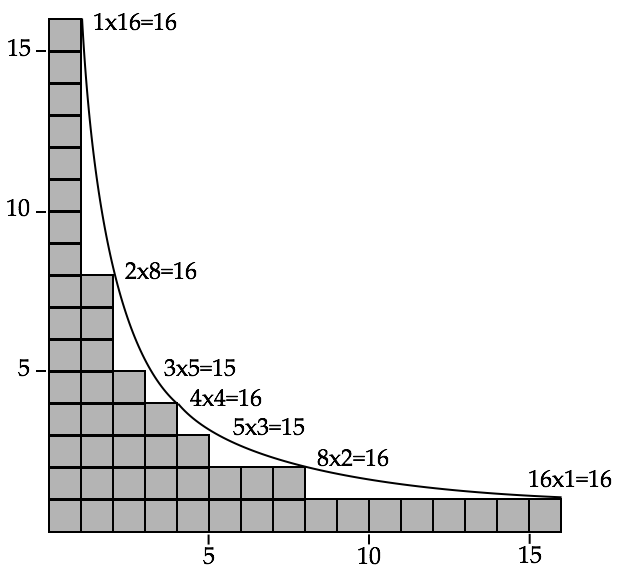
\includegraphics[scale=0.4]{FiguresArithmetic/PairingHyp}
\caption{The aggregate set of positions of tables having $16$ or
    fewer position.  To help the reader understand the figure, we
    include the curve $f(x,y) = xy$ which provides an upper envelope
    for the set.  A careful look at this curve will reveal that it
    touches the set of positions at the points $\langle x,y \rangle
    \in \{ \langle 1,16 \rangle, \ \langle 2,8 \rangle, \ \langle 4,4
    \rangle, \ \langle 8,2 \rangle, \ \langle 16,1 \rangle \}$, but it
    does {\em not} touch the set at the points $\langle x,y \rangle
    \in \{ \langle 3,5 \rangle, \ \langle 5,3 \rangle \}$. 
\label{f.hyp}}
\end{center}
\end{figure}

\subsection{There Are {\em No More} Ordered Pairs than Integers}
\label{sec:cardinality-NxN}

\subsubsection{Comparing infinite sets via cardinalities}
\label{sec:compare-sets-via-card}
\index{cardinality!infinite set}

We have remarked earlier (and will do so again) that one must be very
careful when reasoning about infinite sets.  They can behave in ways
that seem quite contradictory to our experience with finite sets.  One
of the most dramatic instances of this is encountered when we ask
whether the set $\N^+ \times \N^+$ is ``larger'' than the set $\N^+$.
We need to put the word ``larger'' in quotes because we do not know
(yet) what the word means in the setting of infinite sets.  Supplying
a meaning for the word that is at once mathematically tractable and
intuitively plausible was among the seminal contributions of the
19th-century German mathematician and logician Georg
Cantor. \index{Cantor, Georg}


\ignore{\Arny How much do we want to do here?  We can talk about ``$|A| \leq
  |B|$ iff there is an injection from $A$ into $B$''.  We can
  cite---or even prove---the Schroeder-Bernstein Theorem, which
  asserts ``{\em There is a {\em bijection} between sets $A$ and $B$
    iff there is an {\em injection} from $A$ to $B$ and an injection
    from $B$ to $A$.}''.}
    
\ignore{\Denis Yes, develop if not too complicated.}    

Cantor began by seeking an intuitively plausible and mathematically
tractable formal notion that would allow us to verify or refute the
assertion that one infinite set is ``larger'' than another.  He
addressed this question, and related ones, in his groundbreaking study
of the relative ``sizes'' of infinite sets \cite{Cantor74,Cantor78}.
We adapt enough of his formulation to suggest how such issues can be
dealt with mathematically.

We take our lead from finite sets.  Is there a notion of ``bigger''
for finite sets that can be extended to infinite sets?

We begin with a set $A$ of apples and a set $O$ of oranges, together
with the challenge of determining which set is bigger.

\medskip

If sets $A$ and $O$ are both finite, then we can just {\em count} the
number of apples in $A$, call it $a$, and the number of oranges in
$O$, call it $o$, and then compare the sizes of the (nonnegative)
integers $a$ and $o$.  The Trichotomy Laws for integers
(Section~\ref{sec:integers}.A) guarantee that we shall be able to
settle the question.

\noindent
{\em But} we cannot count the elements in an infinite set, so this
approach fails us when we have access to infinitely much fruit!  So we
need another approach.

\medskip

Here is an approach that works for finite sets and that promises to
extend to infinite sets.  Let us assume that we can ``prove''---we
shall explain the word imminently---the following.

For every apple that we extract from set $A$ {\em for the first time},
we can extract an orange from set $O$ {\em for the first time}.  It
will then follow (at least in the finite case), that \\
\hspace*{.35in}{\em There are at least as many oranges as apples!}

\noindent
This is really promising, because there is another way to describe the
fruit-matching process that readily extends to infinite sets.  \\
\hspace*{.35in}{\em There is an injection,\footnote{Recall from
Chapter~\ref{sec:function} that ``{\em injection}'' is synonymous
    with ``{\em one-to-one function}''.}~call it $f$, from $O$ to $A$.} \\
In more formal terms: {\em Every time you pull an apple $\alpha$ from set
  $A$, I pull the orange $f^{-1}(\alpha)$ from $O$.}

\medskip

Inspired by this formulation using injections---and by the work of
Cantor---we craft the following definition.

\noindent
{\em
Given sets $A$ and $O$ (finite or infinite), we say \\
\hspace*{.35in}{\em Set $O$ is at least as big as set $A$, denoted
  $|O| \geq |A|$} \\
precisely when there is an injection from $O$ to $A$.}

\noindent
{\em
Finally, we say that \\
\hspace*{.35in}{\em Sets $O$ and $A$ have the same cardinality,
  denoted $|O| = |A|$} \\
precisely when there is an injection from $O$ to $A$ {\em and} an
injection from $A$ to $O$.}
\index{set cardinality}

\medskip

Finally, back to numbers!

There has always been special interest in comparing the cardinalities of
specific infinite sets with the cardinality of the integers.  This
interest has led to the following pair of adjectives.
\begin{itemize}
\item
A (finite or infinite) set $S$ is {\it countable} \index{countable
  set} \index{set!countable} if $|S| \leq |\N|$.
\item
An infinite set $S$ is {\it uncountable} \index{uncountable set}
\index{set!uncountable} if $|S| \not\leq |\N|$.
\end{itemize}

\subsubsection{Comparing $\N$ and $\N \times \N$ via cardinalities}
\label{sec:compare-NxN-N-via-card}

An obvious first candidate whose cardinality to compare with that of
the integers $\N$ (or $\Z$, or $\N^+$) is the corresponding set of
ordered pairs, $\N \times \N$ (or $\Z \times \Z$, or $\N^+ \times
\N^+$).  Cantor discovered in the 1870s that pairing does not increase
cardinality in infinite sets.  We now prove this for the set $\N$, but
we could easily repeat our argument for $\Z$ or $\N^+$.

\begin{prop}
\label{thm:|NxN|=|N|}
The set $\N \times \N$ is countable:
$|\N \times \N| \ = \ |\N|$.
\end{prop}

\ignore{\Arny So we digress here to address the issue of cardinality.  Should
  we ``assemble'' all such considerations---i.e., $\N \times \N$ and
  $\Q$ and $\R$ into a separate subsection?  I have mixed feelings.}


\begin{proof}
We prove the following propositions in turn.

\medskip

\noindent {\rm (a)} {\em There exists an injection from $\N$ to $\N
  \times \N$.  Therefore, $|\N| \leq |\N \times \N|$; informally, $\N
  \times \N$ is at least as big as $\N$.}

\smallskip

\noindent
Subproposition (a) follows easily from the existence of the following
injection from $\N$ into $\N \times \N$.
\[ (\forall n \in \N) \ [ f(n) \ = \ \langle n,n \rangle]. \]

\medskip

\noindent {\rm (b)} {\em There exists an injection from $\N \times \N$
  to $\N$.  Therefore, $|\N \times \N| \leq |\N|$; informally, $\N$ is
  at least as big as $\N \times \N$.}

\smallskip

\noindent
We establish subproposition (b) by defining an injection from $\N
\times \N$ into $\N$.  We employ a function that is inspired by the
Fundamental Theorem of Arithmetic (Theorem~\ref{thm:Fund-Thm-Arith}).
Specifically, the Theorem assures us that the function
\[ f_2(p,q) \ \eqdef \ 2^p 3^q \]
is an {\em injection} from $\N \times \N$ into $\N$.

Subproposition (a) and (b) prove the result.  \qed
\end{proof}

\medskip

The {\it pairing functions} of Section~\ref{sec:pairing} provide more
interesting alternatives to the preceding proof of
Proposition~\ref{thm:|NxN|=|N|}.  Being {\em bijections} between $\N$
and $\N \times \N$, pairing functions can be adapted to prove any such
proposition {\em in a single step}. 

\medskip

We now present a remarkable theorem that demonstrates that such
single-step proofs of equality of cardinality are {\em always}
available!  There is {\em always} a bijection whenever there exist
paired injections!


\subsubsection{The Schr\"{o}der-Bernstein Theorem}
\label{sec:schroeder-bernstein}

Although sets and their cardinalities are not the major focus of this
chapter, it is worth a short digression to expand on the last remark
in Section~\ref{sec:compare-NxN-N-via-card}.  It is not a coincidence
that there exists both \\
\hspace*{.35in}{\em a bijection between $\N$ and $\N \times \N$} \\
and \\
\hspace*{.35in}{\em an injection from $\N$ to $\N \times \N$ and an
  injection from $\N \times \N$ to $\N$.}

\noindent
The celebrated theorem of Schr\"{o}der and Bernstein,
\index{The Schr\"{o}der-Bernstein Theorem}
\index{Bernstein, Felix}
\index{Schr\"{o}der, Ernst}
which is, alternatively, attributed to (Georg) Cantor and Bernstein, 
\index{The Cantor-Bernstein Theorem}
\index{Cantor, Georg}
tells us that bijections and paired injections always travel together.

\begin{theorem}[The Schr\"{o}der-Bernstein Theorem]
\label{thm.S-B}
Let $S$ and $T$ be (finite or infinite) sets such that there exists an
injection $f: S \rightarrow T$ and an injection $g: T \rightarrow S$.
Then there exists a bijection $h: S \leftrightarrow T$.
\end{theorem}

The theorem has a rather complicated history.  Picking just a few high
points associated with the theorem's namesakes: The theorem was first
stated without proof by Cantor in \cite{Cantor87}.  Roughly a decade
later, Schr\"{o}der provided a flawed proof in \cite{Schroeder98a}.
As reported in \cite{Deiser2010}, Schr\"{o}der soon thereafter
provided a correct proof, as, independently, did Bernstein.

************


\section{Finite Number Systems}
\label{sec:congruences+modular}

The sets that underlie the number systems that we use in most daily
tasks---namely $\N, \Z, \Q$, and $\C$---are infinite: we can always
find a number in each set that is bigger than all the numbers we have
seen thus far.  Indeed, the last two of these sets are ``two-way''
infinite: we can also always find a number in each set that is smaller
than all the numbers we have seen thus
far.\footnote{\label{foot:Pascal}The philosophically inclined reader
might be interested in the essay ``The Two Infinities'' within the
{\it Pens\'{e}es} of the French mathematician-philosopher (or
philosopher-mathematician?) Blaise Pascal \index{Pascal, Blaise},
whose work we shall revisit in Chapter~\ref{sec:binary-operators}.C.}
There do, however, exist several very important situations in which we
use number systems that are {\em finite} and {\em cyclically
  repetitive}.  We mention only two.
\begin{itemize}
\item
The {\em clocks} that we use to indicate daily time are calibrated
into a fixed finite number of major subdivisions, {\em hours}.  We
endow our days with $24$ hours and depending on circumstances, have
our clocks measure each day's time via repeating cycles of either $12$
or $24$ hours.  Once a clock's limit of ($12$ or $24$ hours) has been
reached, it begins its numeration all over---with no memory of the
past.

\item
We typically orient all manner of location specification relative to a
fixed reference point in terms of {\em angles}.  There are two
coexisting, competing systems for such measurement.  One system
subdivides the ``circle'' around the reference point into $360$ {\em
  degrees;} the other subdivides the ``circle'' into $2 \pi$ {\em
  radians}.  For our purposes, the main interesting point is that both
of these systems are {\em cyclically repetitive}.  Once we have
circled the reference point by $360$ degrees (or, equivalently, by $2
\pi$ radians), then we measure further circumnavigation starting over
at $0$ degrees/radians.
\end{itemize}

This section is dedicated to integer-based {\em finite} number systems
that were invented to describe and measure cyclically repetitive
situations such as the two just described.


\subsection{Congruences on Nonnegative Integers}
\label{sec:congruences}

For any positive integer $q \in \N^+$, we denote by $\N_q$ the
$q$-element ``prefix'' of the set $\N$ of nonnegative integers:
\index{$\N_q$: the first $q$ nonnegative integers}
\[ \N_q \ \eqdef \ \{0, 1, \ldots, q-1\} . \]
For nonnegative integers $m, n \in \N$ and positive integer $a \in
\N^+$, we say that {\em $m$ is congruent to $n$ modulo $q$},
\index{integer congruence} \index{congruent to} denoted
\[ m \equiv n \bmod q, \]
precisely when $q \mbox{ divides } |m-n|$.  We call $q$ the {\it
  modulus} of the congruence (relation).
\index{modulus}

\begin{prop}
\label{thm:CONGisEQUIVALENCE-REL}
The relation of congruence modulo a positive integer is an equivalence
relation on the set $\N$ of nonnegative integers.
\end{prop}

\begin{proof}
We verify in turn the three defining properties of an equivalence
relation (see Chapter~\ref{sec:equiv-relation}).  Focus on nonnegative
integers $m$, $n$, and $r$ and an arbitrary positive integer modulus
$q$.

\begin{enumerate}
\item
Congruence modulo $q \in \N^+$ is a {\em symmetric} relation on $\N$.

{\it Verification:}
Because $|m-n| = |n-m|$, the assertions $[q \mbox{ divides } |n-m|]$
and $[q \mbox{ divides } |n-m|]$ must hold simultaneously, i.e.,
either both assertions are true or neither is.

\item
Congruence modulo $q \in \N^+$ is a {\em reflexive} relation on $\N$.

{\it Verification:}
We always have $m \equiv m \bmod q$ because every positive integer
divides $m-m = 0$.

\item
Congruence modulo $q \in \N^+$ is a {\em transitive} relation on $\N$.

{\it Verification:}
Say that $m \equiv n \bmod q$ and $n \equiv r \bmod q$.  The
arithmetic needed to verify that these two congruences imply that $m
\equiv r \bmod q$ breaks down into cases defined by the relative sizes
of $m$, $n$, and $r$.  We supply the details for the case $m > n > r$,
and we leave the other cases as exercises.

Note first that the two assumed conguences can be rewritten as
assertions of divisibility: $q \mbox{ divides } |m-n|$, and $q \mbox{
  divides } |n-r|$.  Therefore, in the chosen case $m > n > $, the
congruences imply that there exist integers $c_1$ and $c_2$ such that:
  \begin{enumerate}
  \item
$c_1 q = m-n$, which implies that $n = m - c_1 q$;
  \item
$c_2 q = n-q$, which implies that $n = q + c_2 q$.
  \end{enumerate}
We therefore have $r-m = (c2-c_1) q$, which means that $m \equiv r
\bmod q$.  In other words, The relation $equiv \bmod q$ is transitive.
\end{enumerate}
The preceding three properties define an equivalence relation, hence,
jointly verify the proposition.
\qed
\end{proof}

\subsection{Finite Number Systems via Modular Arithmetic}
\label{sec:modular}

Once we embellish the sets $\N_q$ with arithmetic operations---namely,
the ``big four'' of addition, subtraction, multiplication, and
division---we shall see why we are able to use the resulting
congruential systems in the same way as their infinite counterparts,
$\N$, $\Z$, and $\Q$.  In the coming subsections, we show that every
set $\N_q$ can ``mimic'' $\N$ and $\Z$ with respect to addition,
subtraction, and multipliciation, but only when $q$ is a prime number
can $\N_q$ ``mimic'' $\Q$ with respect to division.

\subsubsection{Sums, differences, and products exist within $\N_q$}
\label{sec:modular-add-sub-mult}

Our main result in this section demonstrates that every set $\N_q$,
when embellished with the operations addition, subtraction, and
multiplication, is {\em closed}\index{algebraic closure}\index{closure
  under an arithmetic operation} under these operations, in the sense
spelled out in the following result.

\begin{prop}
\label{thm:modular-add-sub-mult}
For every integer $q \in \N^+$ and all $m,n \in \N_q$, the sum $m+n
\bmod q$ and the difference $m-n \bmod q$ and the product $m \cdot n \bmod
q$ exist within $\N_q$.
\end{prop}

\begin{proof}
For the operations of addition and multiplication, the result is true
by definition of congruence modulo $q$: since the sum $m+n$ and the
product $m \cdot n$ exist within $\N^+$, their ``reductions'' modulo
$q$ exist within $\N_q$.  For the case of subtraction, we augment the
preceding sentence with the following equation.  For all $r \in \Z$
\[ q-r \ \equiv \ -r \bmod q. \]
One verifies this equation by noting the following chain of equalities
and congruences (parentheses added to enhance legibility)
\[ (q-r) - (-r) \ \ = \ \ (q-r) + r \ \ = \ \ q \ \ \equiv \ 0 \bmod q. \] 
In all cases, therefore, the result of the operation remains in the set
$\N_q$.
\qed
\end{proof}

We cannot generally add division to the set of operations listed in
Proposition~\ref{thm:modular-add-sub-mult}.  For instance, the
following table shows that the equation 
\[ 2x \ \equiv \ 1 \bmod 6 \]
is not solvable for all $x \in \N_6 \setminus \{0\}$.
\[ \begin{array}{|c|c|}
\hline
x & 2 \cdot x \bmod 6 \\
\hline
\hline
1 & 2 \\
2 & 4 \\
3 & 0 \\
4 & 2 \\
5 & 4 \\
\hline
\end{array}
\]
The next subsection implicitly identifies the modulus $6$'s
non-primality as the culprit in this example.  In fact, the reader can
easily show that {\em $\N_q$ is never closed under the operation of
  division when the modulus $q$ is composite, i.e., nonprime.}


\subsubsection{Quotients exist within $\N_p$ for every prime $p$}
\label{sec:modular-quotientss}

This section considers congruences modulo a prime number.  We begin
with our main result: {\em for every prime number $p$, every nonzero
  $n \in \N_p$ has a {\em multiplicative inverse}}, i.e., an element
$m \in \N_p$ such that $m \cdot n \equiv 1 \bmod
p$. \index{multiplicative inverse} Of course, the existence of
multiplicative inverses allows one to {\em divide} any number in
$\N_p$ by any nonzero number.

\begin{prop}
\label{thm:finite-field}
For every prime number $p$, every nonzero number $n \in \N_p$ has a
multiplicative inverse within $\N_p$.
\end{prop}

\begin{proof}
Our proof combines applications of the Fundamental Theorem of
Arithmetic (Theorem~\ref{thm:Fund-Thm-Arith}) and the Pigeonhole
Principle (Section~\ref{sec:pigeonhole}), alongside a proof by
contradiction.  It thereby exercises many of our important new proof
techniques.

Focus on the set $\N_p$ for some prime $p$.  Let $n$ be any nonzero
number in $\N_p$.  

\begin{lemma}
\label{lem:multiples-in-Zp-unique}
There do {\em not} exist nonzero numbers $m_1$ and $m_2 \neq m_1$ in
$\N_p$ such that $m_1 \cdot n \equiv m_2 \cdot n \bmod p$.
\end{lemma}

\begin{proof} ({\em of Lemma~\ref{lem:multiples-in-Zp-unique}})
Assume for contradiction that there {\em do} exist $m_1$ and $m_2 \neq
m_1$ in $\N_p$ such that $m_1 \cdot n \equiv m_2 \cdot n \bmod p$.
Say, with no loss of generality, that $m_1 > m_2$ within the set $\N$.
We must then have
\begin{equation}
\label{eq:a-forbidden-divisibility}
p \ \mbox{ divides } \ (m_1 - m_2) \cdot n.
\end{equation}
The fact that $p$ is a prime ensures---by
Proposition~\ref{thm:p-divides-onefactor}---that $p$ divides at least
one of the integers $n$ or $(m_1 - m_2)$.  Because both of these
integers belong to $\N_p$, hence lie strictly between $0$ and $p-1$
(within the infinite set $\N$), the divisibility posited in
(\ref{eq:a-forbidden-divisibility}) is impossible!  The lemma follows.
\qed
\end{proof}

Lemma~\ref{lem:multiples-in-Zp-unique} guarantees that all of the
following $p-1$ elements of $\N_p$ are nonzero and distinct:
\[ 1 \cdot n, \ \ 2 \cdot n, \ldots, \ \ (p-1) \cdot n. \]
Because $\N_p$ has precisely $p-1$ nonzero elements, these $p-1$
multiples of $n$ must exhaust these elements.  In other words, some
multiple of $n$, say $c \cdot n$, must equal $1$.  This means that the
number $c \in \N_p$ is $n$'s multiplicative inverse within $\N_p$.
\qed
\end{proof}

\medskip

Of course, once we have multiplicative inverses, we have the operation
of division and, consequently, arbitrary quotients and fractions.  Of
course, fractions within finite number systems such as $\N_p$ are
going to look strange to our eyes, as the following example indicates.

What does the number $7/4$ look like within $\N_5$?  We develop the
answer in steps.

\[ \approx \approx \approx \approx \approx \approx \approx \approx \approx \approx \]
We are able to proceed in the following manner because the relations
($\equiv \bmod q$) are {\em congruences}, \index{congruence relation}
i.e., equivalence relations whose class structures are consistent with
the algebraic structure of the arithmetic systems exemplified by $\Z$,
$\Q$, $\R$, and $\N_p$ under the classical four arithmetic operations.
A full treatment of this topic is beyond the scope of this text.
\[ \approx \approx \approx \approx \approx \approx \approx \approx \approx \approx \]
\begin{enumerate}
\item
The numbers $4, 7 \in \N$ correspond, respectively, to the numbers $4,
2 \in \N_5$.

Verification:
$4 \equiv 4 \bmod 5$, and $7 \equiv 2 \bmod 5$.

\item
The multiplicative inverse of $4$ within $\N_5$ is $4$.

Verification:
$4 \cdot 4 \ = \ 16 \ \equiv 1 \bmod 5$.

\item
THEREFORE, we have the following ``translation'' of the quotient $7/4$:

Within $\N$: \\
the product of $7 \in \N$ by the multiplicative inverse of $4 \in \N$

Within $\N_5$: \\
the product of $2 \in \N_5$ by the multiplicative inverse of $4 \in
\N_5$, which is $4$

\item
the product of $2 \in \N_5$ by $4 \in \N_5$ is $3$.

Verification:
$2 \cdot 4 \ = \ 8 \ \equiv 3 \bmod 5$.
\end{enumerate}
We thus have the unintuitive fact that the rational number $7/4$
corresponds to the number $3 \in \N_6$.

Of course, we do not often perform arbitrary arithmetic within the
finite number systems $\N_p$, so we do not often struggle with the
unfamiliar results of this subsection.  That said, we do sometimes
intermix ``ordinary'' numeration with ``modular'' numeration, as when
we coordinate talk about elapsed time (measured in the ``ordinary''
way) with wall-clock time (which is a ``modular'' system).  So, in
summation, it is worth the effort to understand this seldom-used
material.  Plus, it can be amusing to announce at a party that you can
``prove'' that $1.75 = 3$.

